\section{Architecture}

\begin{figure}[t]
    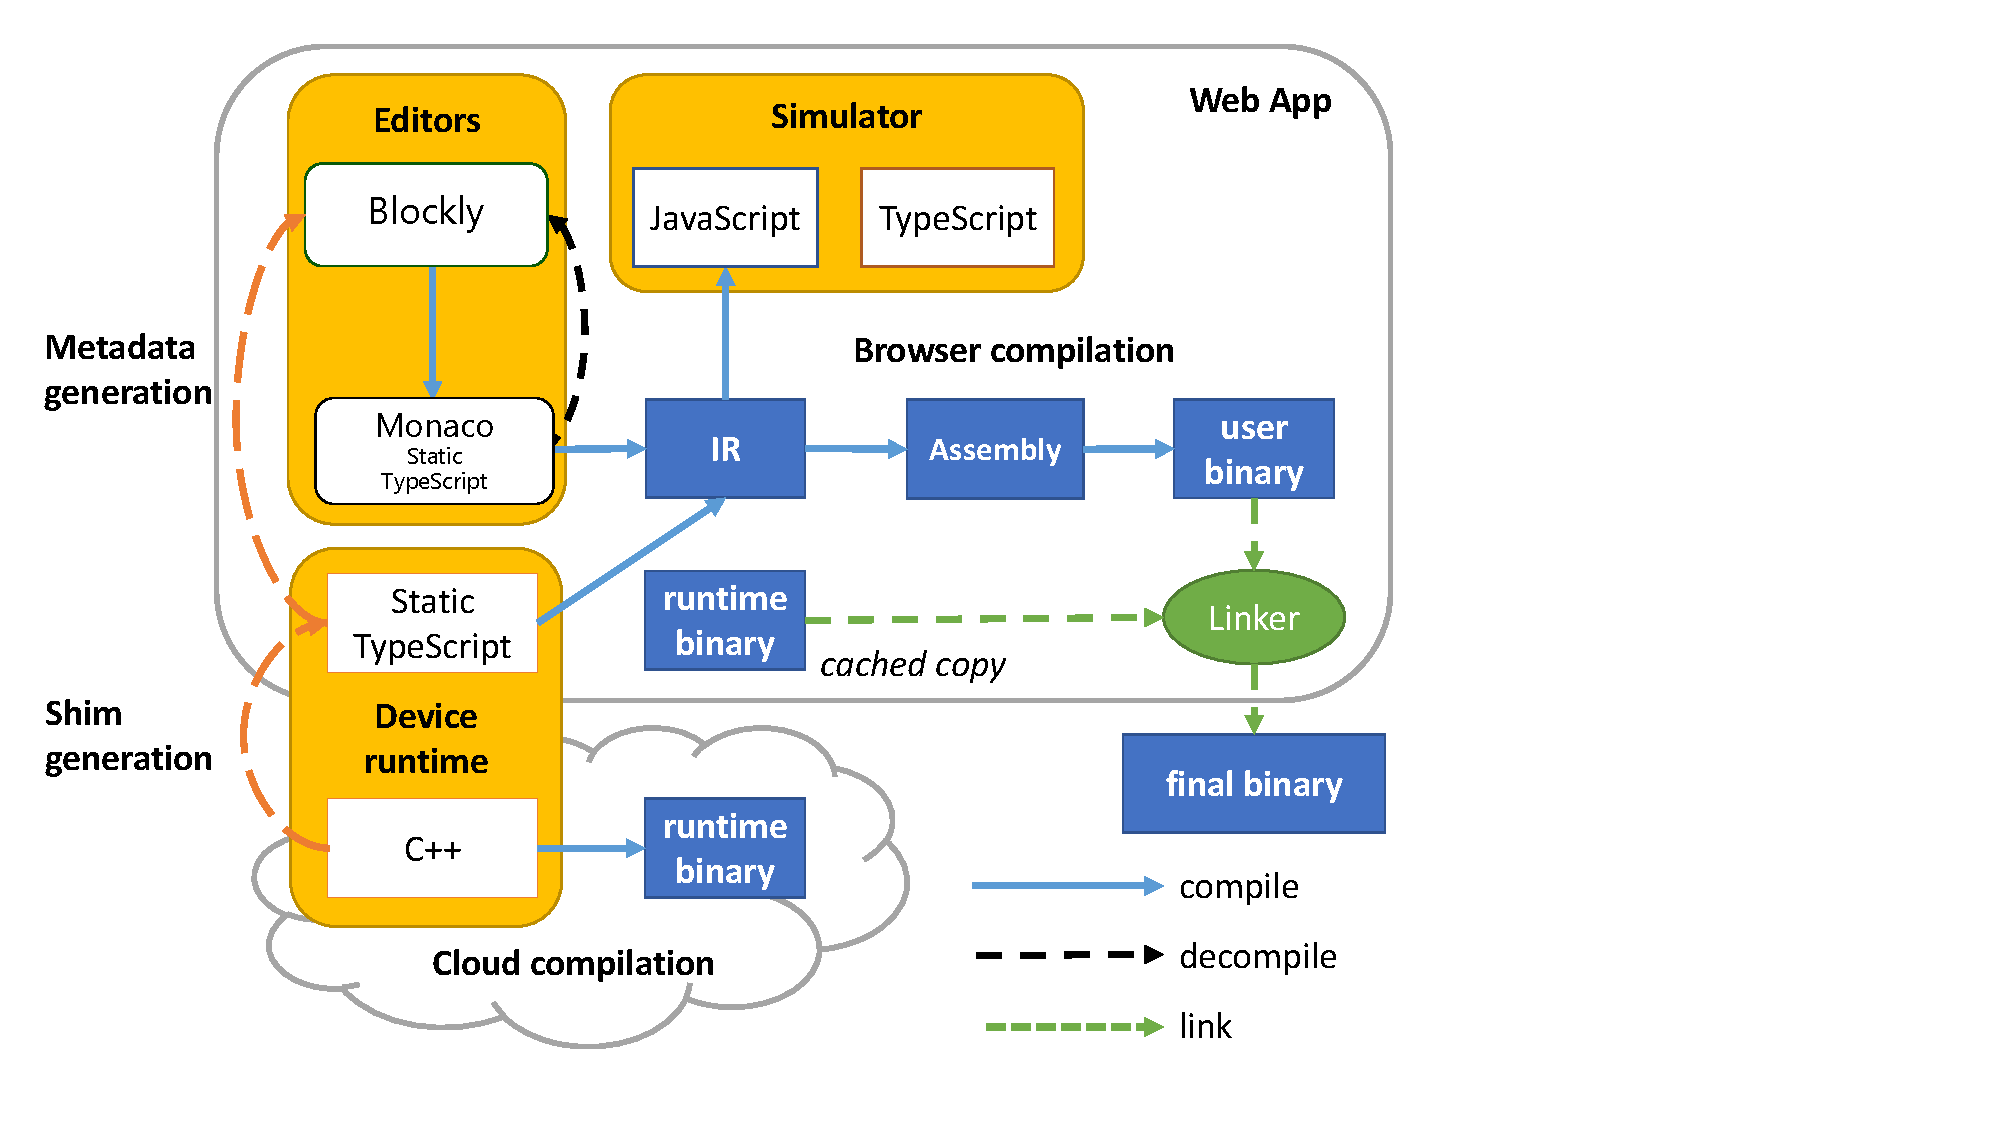
\includegraphics[width=4.8in]{makecodeFig.pdf}
\caption{\label{fig:makecode}\MC web app}
\end{figure}

Currently, due to the low-level nature of MCU programming, additional drivers and software are commonly required to be locally installed in order to program them. In restricted environments, like libraries and schools, safeguards are put in place to protect users and machines from downloading or installing additional software. Further, Internet connections are unreliable in remote locations. These factors create barriers for designing a programming environment suited to a diverse audience. Therefore, a solution is required that can: (1) operate in restricted environments; (2) operate with little, or no internet connectivity; and (3) work on any operating system.

To meet these requirements, we created the \MC web app (Figure~\ref{fig:makecode}), the entry point of the platform. The web app can be accessed from any modern web browser and cached locally for \emph{entirely offline use}. The \MC web app incorporates the open source Blockly (\emph{\href{https://github.com/google/blockly}{blockly}}) and Monaco (\emph{\href{https://github.com/Microsoft/monaco-editor}{monaco-editor}}) editors (upper-left), an in-browser device simulator (upper-right) for testing programs before transferring them to the physical device, as well as \emph{in-browser compilation} of Static TypeScript to machine code and linking against the C++ runtime (\emph{\CON}), pre-compiled (by a cloud service, lower left).

%The statically-typed runtime and type inference on user code allows users to write code that looks like plain JavaScript (see Figure~\ref{fig:example}).

\MC devices appear as USB pen drives when plugged into a computer. After a user has finished developing a program, the compiled binary is ``downloaded'' locally to the users computer and then transferred (flashed) to the MCU (exposed as USB pen drive) by a simple file copy operation. No additional installation is required to program the MCU as drivers for pen drive come pre-installed on many operating systems (MacOS, Windows, Linux, Android, ChromeOS).

These advances enable beginners to get started programming MCUs from any modern web browser, and offer a safe environment for hardware vendors to innovate and add new components using Static TypeScript. All of the platform's components are open source on GitHub (links removed).